\documentclass[letterpaper,times]{IONconf-v2}

% IONconf-v2 (ION's NAVIGATION template, LaTexTemplate.zip) already loads amsmath, graphicx,
% booktabs, tabularray, tikz, xcolor and biblatex-apa with natbib=true.
\usepackage{bm}
\setcounter{MaxMatrixCols}{20}
\usepackage{siunitx}
\usepackage{algorithm}
\usepackage{algpseudocode}
\usepackage{multirow}
\usetikzlibrary{arrows.meta,positioning,fit,calc}
\sisetup{group-separator={,},group-minimum-digits=4}

\addbibresource{references.bib}

\usepackage[hidelinks]{hyperref}
\usepackage[capitalize,noabbrev]{cleveref}

\graphicspath{{figures/}}

% Numbers quoted in running text, generated by scripts/build_tables.py.
\newcommand{\numdatasethours}{55.3}
\newcommand{\numdatasetkm}{4{,}338}
\newcommand{\numdedicatedekfbothbetter}{24}
\newcommand{\numdedicatedekfbothdmed}{46.7}
\newcommand{\numdedicatedekfbothn}{27}
\newcommand{\numdedicatedekfbothp}{\(<10^{-3}\)}
\newcommand{\numdedicatedekfbothratio}{0.890}
\newcommand{\numdedicatedekfbothworse}{3}
\newcommand{\numdedicatedekfgravbetter}{8}
\newcommand{\numdedicatedekfgravdmed}{3.6}
\newcommand{\numdedicatedekfgravn}{27}
\newcommand{\numdedicatedekfgravp}{0.17}
\newcommand{\numdedicatedekfgravratio}{1.005}
\newcommand{\numdedicatedekfgravworse}{19}
\newcommand{\numdedicatedekfmagbetter}{25}
\newcommand{\numdedicatedekfmagdmed}{48.0}
\newcommand{\numdedicatedekfmagn}{27}
\newcommand{\numdedicatedekfmagp}{\(<10^{-3}\)}
\newcommand{\numdedicatedekfmagratio}{0.891}
\newcommand{\numdedicatedekfmagworse}{2}
\newcommand{\numdedicatedrbpfbothbetter}{18}
\newcommand{\numdedicatedrbpfbothdmed}{93{,}107.4}
\newcommand{\numdedicatedrbpfbothn}{25}
\newcommand{\numdedicatedrbpfbothp}{0.22}
\newcommand{\numdedicatedrbpfbothratio}{0.875}
\newcommand{\numdedicatedrbpfbothworse}{7}
\newcommand{\numdedicatedrbpfgravbetter}{11}
\newcommand{\numdedicatedrbpfgravdmed}{45{,}017.9}
\newcommand{\numdedicatedrbpfgravn}{25}
\newcommand{\numdedicatedrbpfgravp}{0.37}
\newcommand{\numdedicatedrbpfgravratio}{1.157}
\newcommand{\numdedicatedrbpfgravworse}{14}
\newcommand{\numdedicatedrbpfmagbetter}{10}
\newcommand{\numdedicatedrbpfmagdmed}{38{,}029.5}
\newcommand{\numdedicatedrbpfmagn}{25}
\newcommand{\numdedicatedrbpfmagp}{0.41}
\newcommand{\numdedicatedrbpfmagratio}{1.088}
\newcommand{\numdedicatedrbpfmagworse}{15}
\newcommand{\numdedicatedukfbothbetter}{26}
\newcommand{\numdedicatedukfbothdmed}{43.5}
\newcommand{\numdedicatedukfbothn}{27}
\newcommand{\numdedicatedukfbothp}{\(<10^{-3}\)}
\newcommand{\numdedicatedukfbothratio}{0.899}
\newcommand{\numdedicatedukfbothworse}{1}
\newcommand{\numdedicatedukfgravbetter}{8}
\newcommand{\numdedicatedukfgravdmed}{4.5}
\newcommand{\numdedicatedukfgravn}{27}
\newcommand{\numdedicatedukfgravp}{0.049}
\newcommand{\numdedicatedukfgravratio}{1.011}
\newcommand{\numdedicatedukfgravworse}{19}
\newcommand{\numdedicatedukfmagbetter}{26}
\newcommand{\numdedicatedukfmagdmed}{45.3}
\newcommand{\numdedicatedukfmagn}{27}
\newcommand{\numdedicatedukfmagp}{\(<10^{-3}\)}
\newcommand{\numdedicatedukfmagratio}{0.901}
\newcommand{\numdedicatedukfmagworse}{1}
\newcommand{\numekfdegradedmedian}{440.4}
\newcommand{\numekfdegradedn}{27}
\newcommand{\numekfdegradedvmedian}{23.4}
\newcommand{\numekffullmedian}{4.1}
\newcommand{\numekffulln}{27}
\newcommand{\numekffullvmedian}{1.6}
\newcommand{\numphoneekfbothbetter}{8}
\newcommand{\numphoneekfbothdmed}{0.4}
\newcommand{\numphoneekfbothn}{27}
\newcommand{\numphoneekfbothp}{0.46}
\newcommand{\numphoneekfbothratio}{1.001}
\newcommand{\numphoneekfbothworse}{19}
\newcommand{\numphoneekfgravbetter}{7}
\newcommand{\numphoneekfgravdmed}{0.5}
\newcommand{\numphoneekfgravn}{27}
\newcommand{\numphoneekfgravp}{0.18}
\newcommand{\numphoneekfgravratio}{1.001}
\newcommand{\numphoneekfgravworse}{20}
\newcommand{\numphoneekfmagbetter}{12}
\newcommand{\numphoneekfmagdmed}{0.0}
\newcommand{\numphoneekfmagn}{27}
\newcommand{\numphoneekfmagp}{0.93}
\newcommand{\numphoneekfmagratio}{1.000}
\newcommand{\numphoneekfmagworse}{15}
\newcommand{\numphonerbpfbothbetter}{13}
\newcommand{\numphonerbpfbothdmed}{16{,}894.9}
\newcommand{\numphonerbpfbothn}{25}
\newcommand{\numphonerbpfbothp}{0.83}
\newcommand{\numphonerbpfbothratio}{0.950}
\newcommand{\numphonerbpfbothworse}{12}
\newcommand{\numphonerbpfgravbetter}{14}
\newcommand{\numphonerbpfgravdmed}{50{,}720.4}
\newcommand{\numphonerbpfgravn}{25}
\newcommand{\numphonerbpfgravp}{0.44}
\newcommand{\numphonerbpfgravratio}{0.890}
\newcommand{\numphonerbpfgravworse}{11}
\newcommand{\numphonerbpfmagbetter}{12}
\newcommand{\numphonerbpfmagdmed}{1{,}564.1}
\newcommand{\numphonerbpfmagn}{26}
\newcommand{\numphonerbpfmagp}{0.35}
\newcommand{\numphonerbpfmagratio}{1.024}
\newcommand{\numphonerbpfmagworse}{14}
\newcommand{\numphoneukfbothbetter}{8}
\newcommand{\numphoneukfbothdmed}{0.5}
\newcommand{\numphoneukfbothn}{27}
\newcommand{\numphoneukfbothp}{0.14}
\newcommand{\numphoneukfbothratio}{1.001}
\newcommand{\numphoneukfbothworse}{19}
\newcommand{\numphoneukfgravbetter}{9}
\newcommand{\numphoneukfgravdmed}{0.4}
\newcommand{\numphoneukfgravn}{27}
\newcommand{\numphoneukfgravp}{0.13}
\newcommand{\numphoneukfgravratio}{1.001}
\newcommand{\numphoneukfgravworse}{18}
\newcommand{\numphoneukfmagbetter}{13}
\newcommand{\numphoneukfmagdmed}{0.0}
\newcommand{\numphoneukfmagn}{27}
\newcommand{\numphoneukfmagp}{0.86}
\newcommand{\numphoneukfmagratio}{1.000}
\newcommand{\numphoneukfmagworse}{14}
\newcommand{\numrbpfdegradedmedian}{664.6~km}
\newcommand{\numrbpfdegradedn}{25}
\newcommand{\numrbpfdegradedvmedian}{409.5}
\newcommand{\numrbpffullmedian}{1.9}
\newcommand{\numrbpffulln}{27}
\newcommand{\numrbpffullvmedian}{1.6}
\newcommand{\numsensekfcount}{1}
\newcommand{\numsensekfmaxm}{261}
\newcommand{\numsensekfmedianpct}{0}
\newcommand{\numsensekfn}{27}
\newcommand{\numsensrbpfcount}{22}
\newcommand{\numsensrbpfmaxm}{915{,}818}
\newcommand{\numsensrbpfmedianpct}{20}
\newcommand{\numsensrbpfn}{25}
\newcommand{\numsensukfcount}{0}
\newcommand{\numsensukfmaxm}{0}
\newcommand{\numsensukfmedianpct}{0}
\newcommand{\numsensukfn}{27}
\newcommand{\numukfdegradedmedian}{430.4}
\newcommand{\numukfdegradedn}{27}
\newcommand{\numukfdegradedvmedian}{24.0}
\newcommand{\numukffullmedian}{4.0}
\newcommand{\numukffulln}{27}
\newcommand{\numukffullvmedian}{1.6}

\newcommand{\bounddegradedkm}{0.44}
\newcommand{\boundgradgrav}{1.44}
\newcommand{\boundgradmag}{6.37}
\newcommand{\boundreqgrav}{0.6}
\newcommand{\boundreqmag}{2.8}
\newcommand{\boundscaleadxl}{38}
\newcommand{\boundscalephonegrav}{91}
\newcommand{\boundscalephonemag}{1{,}183}
\newcommand{\boundscalermthree}{0.6}

\newcommand{\rbpfdiagcrossed}{24}
\newcommand{\rbpfdiagcrossingmin}{6}
\newcommand{\rbpfdiagdrives}{25}
\newcommand{\rbpfdiagerrorkm}{879}
\newcommand{\rbpfdiagratio}{14{,}416}
\newcommand{\rbpfdiagsigmam}{74}


\articletype{Original paper}%
\journalname{NAVIGATION}

\title{Gravity and Magnetic Anomaly Aiding of a Smartphone-Grade Inertial Navigation System under Degraded GNSS: A Paired Evaluation of Kalman and Particle Filters}

\author[1]{James Brodovsky*}
\author[1]{Philip Dames}

\authormark{BRODOVSKY \textsc{and} DAMES}

\address[1]{Department of Mechanical Engineering, Temple University, Philadelphia, Pennsylvania, USA}

\corres{*James Brodovsky, Temple University, Philadelphia, PA, USA.\\ \email{jbrodovsky@temple.edu}}

\begin{document}

\abstract[Abstract]{Gravity and magnetic anomaly maps offer a position reference that cannot be jammed, and a vehicle-mounted smartphone already carries both an accelerometer and a magnetometer. This paper asks whether those readings, or the readings of comparably priced dedicated sensors, reduce the error of a smartphone-grade inertial navigation system (INS) when GNSS fixes arrive only once per minute with correlated errors. An extended Kalman filter (EKF), an unscented Kalman filter (UKF), and a Rao-Blackwellized particle filter (RBPF) after Canciani and Raquet are evaluated on 27 drives totalling \numdatasetkm~km and \numdatasethours~h, each aided run paired with the same filter's unaided run on an identical, seeded measurement stream. The paper corrects and supersedes two earlier conference papers by the authors, whose reported gains arose from unit errors in the anomaly measurement and from comparisons against diverged baselines. With the corrected models, the smartphone's own readings provide no measurable benefit to either Kalman filter (median RMSE ratio 1.000 to 1.001), because the operating system pins the gravity norm to a device constant and the magnetometer is dominated by the vehicle's field, giving signal-to-noise ratios of 0.13 and 0.01 against the maps. Replacing only those readings with a simulated RM3100 magnetometer reduces the median error by about 10\% (ratios \numdedicatedekfmagratio{} for the EKF and \numdedicatedukfmagratio{} for the UKF, improving \numdedicatedekfmagbetter{} and \numdedicatedukfmagbetter{} of 27 drives), whereas a simulated ADXL355 used as a gravimeter does not help. The RBPF loses track under the 60-s GNSS schedule with or without aiding. The quality of the anomaly measurement relative to the map signal, rather than the estimator or the inertial sensor, decides whether aiding helps.
}

\keywords{alternative navigation, geophysical navigation, magnetic anomaly navigation, gravity anomaly navigation, MEMS inertial navigation, particle filter, unscented Kalman filter, GNSS degradation}

\maketitle

\section{Introduction}
\label{sec:introduction}

An inertial navigation system (INS) integrates specific force and angular rate into position, and its error grows without bound unless an external position or velocity reference arrests it. On most platforms that reference is GNSS, whose low received power makes it easy to deny by jamming, to corrupt by spoofing, and to lose in urban canyons, under foliage, indoors, and underwater \citep{humphreys2008, divis2013gps}. How quickly the INS error grows once GNSS is lost is set by the grade of the inertial sensor. A navigation-grade system coasts for tens of minutes before accumulating 100~m of error; the consumer-grade micro-electro-mechanical systems (MEMS) IMU found in a smartphone, a small drone, or a low-cost autonomous vehicle crosses the same threshold in under a minute \citep{groves_ch14}. For the platforms that carry such sensors, which vastly outnumber those carrying navigation-grade instruments, an alternative aiding source must be available continuously, everywhere the platform operates, and at a cost commensurate with the platform itself.

Map-matching against the Earth's geophysical fields is one of the few alternatives that is present everywhere and at all times without depending on infrastructure. Terrain- and bathymetry-aided navigation are the most mature members of that family \citep{baker1977terrain, williams2001towards_tan, donovan2012}, but they require an active emission. Gravity and magnetic anomalies are sensed passively, and anomaly-aided navigation has been demonstrated with gravimeters on submarines and ground vehicles \citep{jircitano1991gravity, kamgar1999vehicle} and with survey magnetometers on aircraft \citep{canciani2016absolute, canciani2017airborne}. Every such demonstration, however, pairs a tactical- or navigation-grade INS with a specialized survey instrument. Whether the technique survives the replacement of both halves of that pairing, a MEMS IMU in place of the high-grade inertial system and commodity sensing in place of the survey instrument, has not been established.

This paper addresses that question with three estimators on one body of data. An extended Kalman filter (EKF), an unscented Kalman filter (UKF), and a Rao-Blackwellized particle filter (RBPF) in the form of \citet{canciani2017airborne} are each aided with gravity anomaly, magnetic anomaly, or both, and each aided run is paired with the same filter's unaided run on the same drive. All three filters share one strapdown mechanization and one seeded measurement stream, so that the anomaly measurement is the only difference within a pair. The drives are the 27 trajectories of the MEMS-Nav dataset, \numdatasetkm~km and \numdatasethours~h of smartphone recordings on public roads in the Mid-Atlantic United States \citep{mems-nav-dataset}. GNSS is degraded to one fix per minute with correlated position and velocity errors, a regime in which the unaided EKF's median horizontal error is \numekfdegradedmedian~m against \numekffullmedian~m with full GNSS. The anomaly observations come from two sources: the gravity and magnetic readings that the smartphone itself records, and, as a control, simulated readings of two low-cost dedicated sensors substituted for them with everything else held fixed.

\subsection{Relation to Earlier Work by the Authors}

Preliminary versions of this work were presented at the 2026 ION International Technical Meeting, with a UKF \citep{anom-ukf}, and at the 2026 ION Pacific PNT Meeting, with an RBPF \citep{anom-pf}. Both reported that the smartphone's gravity and magnetic readings reduced navigation error, by tens to hundreds of meters for the UKF and by more than 1{,}500~km for the RBPF. Those results do not hold. An audit of the software found that the anomaly observation was formed with unit errors that left it unrelated to the maps, and that the comparisons were made against baselines that had themselves diverged. \Cref{sec:corrections} sets out each defect and its effect. This paper replaces the conference results in full: it uses the corrected measurement models, a larger dataset, a common GNSS degradation for every run, a paired statistical design, and a third estimator. Its conclusions about the smartphone sensors are the opposite of those reported earlier.

\subsection{Contributions}

The contributions of this paper are as follows.
\begin{enumerate}
  \item A paired evaluation of EKF, UKF, and RBPF anomaly aiding of a consumer-grade MEMS INS on 27 ground-vehicle drives, in which every filter receives an identical, reproducible measurement stream and each aided run is scored against its own unaided counterpart.
  \item A corrected formulation of the gravity and magnetic anomaly observations, with an error model measured from the data against the maps, and an explicit account of the defects that invalidated the authors' earlier conference results.
  \item A null result for the smartphone's own sensors and its mechanism: the operating system pins the reported gravity norm to a device constant, and the vehicle's own magnetic field dominates the magnetometer, so both observations have signal-to-noise ratios far below one against the maps.
  \item A controlled test with simulated dedicated sensors showing that a \$25 magnetometer makes magnetic aiding consistently beneficial for both Kalman filters with the same consumer-grade IMU, whereas a \$77 MEMS accelerometer used as a gravimeter does not, and that the size of the benefit is consistent with a per-update localization bound.
  \item A negative result for the particle filter, which loses track under once-per-minute GNSS with or without aiding, with a diagnosis of the failure.
  \item An open-source implementation \citep{strapdown-rs} and dataset with which every number in this paper can be regenerated.
\end{enumerate}

The remainder of the paper is organized as follows. \Cref{sec:corrections} documents the corrections to the conference results. \Cref{sec:navigation} describes the shared mechanization, the GNSS degradation model, and the three filters. \Cref{sec:geophysical} develops the anomaly measurement models and their error models. \Cref{sec:experiment} describes the data and the experimental design, and \Cref{sec:results} the results. \Cref{sec:discussion} discusses the sensor requirement that the results imply, the behavior of the particle filter, and the limitations of the study, and \Cref{sec:conclusion} concludes.

\section{Corrections to the Conference Results}
\label{sec:corrections}

This section documents why the results of \citet{anom-ukf} and \citet{anom-pf} are withdrawn. Each defect below was confirmed by inspecting the software revisions used to produce those papers, and each has since been fixed in \texttt{strapdown-rs} with a regression test that fails if it is reintroduced. \Cref{tab:conference-vs-journal} summarizes how the experiment of this paper differs from those of the conference papers.

\subsection{Anomaly Observations That Carried No Map Information}

The gravity anomaly observation was formed as \(\lVert\mathbf{g}_\text{obs}\rVert - \gamma - E\) in m/s\(^2\) and then differenced against a map in mGal, a factor of \(10^5\) apart. Normal gravity \(\gamma\) was evaluated with the latitude in radians passed to a function that expects degrees, which places every observation at the equator and introduces an error of about \(-2{,}100\)~mGal at 40\(^\circ\)~N, and at the ellipsoid surface rather than at the observation height, which omits the free-air gradient of 0.31~mGal/m. The E\"{o}tv\"{o}s correction \(E\) was subtracted rather than added, doubling rather than removing the motion term, and used the radius of the parallel in place of the radii of curvature. The magnetic anomaly observation subtracted the World Magnetic Model (WMM) total intensity expressed in tesla, about \(5\times10^{-5}\), from an observed intensity in microtesla, so that no core field was removed, and differenced the result against a map in nanotesla.

In both channels the quantity passed to the filter was therefore a number of order \(10^{-2}\) to \(10^{1}\) in the units of a map whose anomalies span tens to hundreds of units. The observation was effectively constant, and each update pulled the solution toward positions at which the map value plus the bias state matched that constant. The residual statistics reported in the conference papers, a magnetic standard deviation of 41{,}303~nT among them, describe this defective observation, not the sensors.

\subsection{Comparisons Against Baselines That Differed or Had Diverged}

In both conference papers the aided and unaided runs were produced by different code paths: the aided runs by an event-stream builder in the geophysical module that had diverged from the one used for the unaided runs. In the software used for \citet{anom-pf}, the unaided stream contained a magnetometer heading update that the aided stream lacked, so the two runs differed in more than the anomaly measurement. The GNSS error model was parameterized per fix rather than per unit time, which made its steady-state wander depend on the fix interval.

The RBPF paper's headline improvement of about 1{,}566~km is a difference against an unaided RBPF whose own mean horizontal RMSE over the 21 drives was about 1{,}572~km, larger than any of the routes. Against the unaided UKF of the same paper, whose mean RMSE was about 7.1~km, the aided RBPF was better on 11 to 14 of 21 drives by RMSE and worse by per-drive median error. Neither comparison isolates the effect of the anomaly measurement. The RBPF of that paper also differed from the one evaluated here: each particle carried its own Kalman filter over 14 linear states including IMU biases, resampling was triggered by the effective sample size, and nothing prevented the cloud from collapsing onto a single ancestor.

\begin{table}[htb]
  \caption{The Experiment of This Paper Compared with Those of the Conference Papers}
  \label{tab:conference-vs-journal}
  \centering
  \small
  \begin{tabular}{p{0.20\textwidth}p{0.35\textwidth}p{0.37\textwidth}}
    \toprule
    & Conference papers \citep{anom-ukf, anom-pf} & This paper \\
    \midrule
    Drives & 13 (UKF) and 21 (RBPF) & 27, all filters \\
    Record rate & 1~Hz & 10~Hz inertial, about 1~Hz GNSS \\
    GNSS degradation & AR(1) per fix, \(\rho\) = 0.99 / 0.95, \(\sigma\) = 5~m / 5~m/s, \(R\) inflated by \(15^2\) & One fix per 60~s; first-order Gauss--Markov errors, 35~m / 500~s and 1.5~m/s / 100~s; \(R\) inflated by \(5^2\) \\
    Gravity observation & Unit, latitude, height and E\"{o}tv\"{o}s defects (above) & \Cref{eqn:gravity-anomaly-obs} \\
    Magnetic observation & Raw intensity in \(\mu\)T, no core field removed & \Cref{eqn:magnetic-anomaly-obs}, WMM2020/2025 \\
    Anomaly error model & Statistics of the defective observation & Measured against the maps (\Cref{tab:error-model}) \\
    Filters & UKF; RBPF with a Kalman filter per particle & EKF, UKF; RBPF after \citet{canciani2017airborne} \\
    Comparison & Aided vs.\ separately built unaided runs & Aided vs.\ the same filter's unaided run on an identical stream; bootstrap CI and Wilcoxon test \\
    Control experiment & None & Simulated dedicated sensors (\Cref{sec:dedicated-sensors}) \\
    \bottomrule
  \end{tabular}
\end{table}

\subsection{What Survives}

The software framework, the dataset, and the question posed by the conference papers stand. Their conclusions do not: with corrected observations the smartphone's sensors provide no benefit to any filter (\Cref{sec:results-phone}), and the particle filter, far from being the best-suited estimator, does not maintain a solution under the degraded GNSS scenario used here (\Cref{sec:results-rbpf}). Readers who have cited the conference papers for a quantitative benefit of smartphone-based anomaly aiding should cite this paper instead.

\section{Navigation System}
\label{sec:navigation}

All three filters share one strapdown mechanization, one set of GNSS, barometric, and heading measurement models, and one measurement stream, so that a comparison between filters, or between an aided run and its unaided counterpart, isolates the estimator or the anomaly measurement. Positions are WGS~84 geodetic latitude \(L\), longitude \(\lambda\), and ellipsoidal height \(h\); velocities are resolved in the local north--east--down frame; attitude is held as a direction cosine matrix \(\mathbf{C}_b^n\) and reported as roll, pitch, and yaw.

\subsection{Mechanization and Aiding Measurements}

The mechanization is the local-navigation-frame strapdown algorithm of \citet[Sections~5.4--5.5]{groves_ch5}: the attitude update integrates the bias-corrected angular rate less the Earth and transport rates, the velocity update resolves the bias-corrected specific force into the navigation frame and adds the Somigliana normal gravity and the Coriolis and transport-rate terms, and position is integrated with the meridian and transverse radii of curvature. The Kalman filters estimate the fifteen states
\begin{equation}
  \mathbf{x} = \begin{bmatrix} L & \lambda & h & v_N & v_E & v_D & \phi & \theta & \psi & \mathbf{b}_a^\top & \mathbf{b}_g^\top \end{bmatrix}^\top,
  \label{eqn:state}
\end{equation}
where \(\mathbf{b}_a\) and \(\mathbf{b}_g\) are the accelerometer and gyroscope biases, together with a barometric-bias state that every run in this paper carries and, when aided, one map-bias state per anomaly channel (\Cref{sec:geophysical}).

Three aiding sources are common to every run. GNSS is loosely coupled as a five-element observation of latitude, longitude, height, and north and east velocity, with a diagonal covariance built from the receiver's reported accuracies. The barometer supplies a relative altitude referenced to the first GNSS height, and the magnetometer supplies a once-per-second heading observation with a standard deviation of 0.2~rad. The heading observation is common to the aided and unaided runs, and so does not affect their comparison; its accuracy on this data is poor (\Cref{sec:limitations}).

\subsection{GNSS Degradation}

GNSS degradation is applied by replaying the recorded fixes through a seeded scheduler and fault model before any filter sees them, so that every filter and every aiding configuration receives an identical corrupted stream. The scheduler delivers one fix every \(T = 60\)~s. The fault model adds independent first-order Gauss--Markov errors to the north and east components of each delivered position and velocity,
\begin{equation}
  \mathbf{e}_{k+1} = e^{-\Delta t_k/\tau}\,\mathbf{e}_k + \sigma\sqrt{1 - e^{-2\Delta t_k/\tau}}\;\mathbf{w}_k, \qquad \mathbf{w}_k \sim \mathcal{N}(\mathbf{0}, \mathbf{I}_2),
  \label{eqn:gauss-markov}
\end{equation}
with \(\sigma = 35\)~m and \(\tau = 500\)~s for position and \(\sigma = 1.5\)~m/s and \(\tau = 100\)~s for velocity, where \(\Delta t_k\) is the interval between delivered fixes. Specifying the process by a steady-state standard deviation and a correlation time, rather than by a per-fix coefficient, makes its statistics independent of the fix interval. The receiver's reported standard deviations are inflated by a factor of five, so that the filter is told the fixes are degraded. Under this schedule the unaided EKF's median horizontal error rises from \numekffullmedian~m to \numekfdegradedmedian~m (\Cref{sec:results-baselines}).

\subsection{Extended Kalman Filter}
\label{sec:ekf}

The EKF propagates the full state through the mechanization and its covariance through the first-order discretization \(\mathbf{I} + \mathbf{F}\Delta t\) of the local-navigation-frame error-state model of \citet[Eqs.~14.63--14.71]{groves_ch14}, reordered position-first. Because the state holds Euler angles while Groves' attitude error is a rotation vector, every block that touches attitude is converted through the Euler-rate matrix \(\mathbf{E}(\bm{\Phi})\), whose columns are the navigation-frame directions of the roll, pitch, and yaw axes; without that conversion the filter diverged during development. The process noise is \(\mathbf{Q}_k = \mathbf{Q}_c\,\Delta t\) with the spectral densities of \Cref{tab:filter-settings}. The measurement update is the standard EKF update with the Jacobians of the GNSS, barometric, heading, and anomaly models.

\subsection{Unscented Kalman Filter}
\label{sec:ukf}

The UKF carries the same states, process noise, and measurement models, and replaces linearization by the scaled unscented transform \citep{ukf-1, ukf-2, ukf-4}. Its \(2n+1\) sigma points (35 with one anomaly channel, 37 with two) are propagated through the full mechanization, with attitude perturbed on the rotation manifold rather than in Euler angles. The scaling parameter is \(\alpha = 0.1\), with \(\beta = 2\) and \(\kappa = 0\); the textbook \(\alpha = 10^{-3}\) produces a central weight of order \(-10^{6}\) for this state dimension and loses about six significant digits per step to cancellation. For a measurement that is linear in the state the UKF update coincides with the EKF update, so the two filters differ chiefly in propagation and in the anomaly update, where the map enters nonlinearly.

\subsection{Rao-Blackwellized Particle Filter}
\label{sec:rbpf}

The RBPF is the marginalized particle filter of \citet{schon2005marginalized} in the form that \citet{canciani2017airborne} applied to airborne magnetic anomaly navigation. It is an error-state filter around a single nominal trajectory mechanized from every IMU sample. The vertical channel of the nominal is stabilized inside the mechanization by a third-order barometer loop with all three poles at \(-1/\tau_\text{loop}\), so barometric readings feed the loop rather than the filter. The particles sample only the horizontal position error, and every other error state is linear and is carried by a Kalman filter whose covariance all particles share:
\begin{equation}
  \delta\mathbf{x}_n = \begin{bmatrix} \delta L & \delta\lambda \end{bmatrix}^\top, \qquad
  \delta\mathbf{x}_l = \begin{bmatrix} \delta h & \delta\mathbf{v}^\top & \bm{\varepsilon}^\top & \delta h_a & \delta\hat{a} & V_1 & c_1 & \cdots & V_m & c_m \end{bmatrix}^\top,
  \label{eqn:rbpf-partition}
\end{equation}
where \(\bm{\varepsilon}\) is the navigation-frame tilt, \(\delta h_a\) and \(\delta\hat{a}\) are the barometer-loop errors, and each of the \(m\) map channels contributes a first-order Gauss--Markov bias variation \(V_k\) and a random constant \(c_k\). With one map channel this is the thirteen-state filter of the original paper. Like that filter, and unlike the EKF and UKF, it carries no IMU bias states; adding them to \(\delta\mathbf{x}_l\) made the filter diverge on the degraded-GNSS drives.

Following the original Algorithm~1, the error-state transition and process noise are accumulated over the IMU samples between measurements and applied once per measurement epoch. Each particle's horizontal draw is treated as a virtual observation of the linear states, which keeps each particle's velocity and tilt consistent with the horizontal trajectory it represents. Every measurement other than the barometer reweights the particles by the likelihood with the linear states marginalized, \(\log w^i \leftarrow \log w^i - \frac{1}{2}(\mathbf{r}^i)^\top\mathbf{S}^{-1}\mathbf{r}^i\) with \(\mathbf{S} = \mathbf{C}\mathbf{P}\mathbf{C}^\top + \mathbf{R}\), and moves the linear states with a gain shared by the cloud and a Joseph-form covariance update. The weighted-mean error is then fed back into the nominal, and the cloud is resampled systematically after every update.

\Cref{tab:rbpf-departures} lists where the implementation departs from \citet{canciani2017airborne}. Two departures were forced by the data. The paper runs a navigation-grade INS open loop; on MEMS data the loop must be closed. The paper also sets the horizontal process noise to zero (its eq.~19). With zero noise each time update is a noiseless observation of the velocity and tilt errors, which moves their uncertainty out of the shared covariance and into the spread of the particles, where resampling on a meter-level GNSS fix discards it; on a reference drive the conditional velocity uncertainty fell to millimeters per second and the solution ran 17~km off, whereas 1~m/\(\sqrt{\text{s}}\) held it to 3.8~m.

\begin{table}[htb]
  \caption{Departures of the RBPF from \citet{canciani2017airborne}}
  \label{tab:rbpf-departures}
  \centering
  \small
  \begin{tabular}{p{0.27\textwidth}p{0.66\textwidth}}
    \toprule
    Departure & Reason \\
    \midrule
    Closed loop & The weighted-mean error is fed back into the nominal after every update; a MEMS nominal cannot be run open loop. \\
    Discrete WGS~84 transition & The rotation-vector error transition of \citet{groves_ch14} replaces the spherical-Earth Pinson matrices. \\
    Barometer loop completed & Gains and altitude feedback, not printed in the paper, are those of the standard third-order loop \citep{titterton2004strapdown}. \\
    Additional sensors & GNSS position and velocity and magnetometer heading pass through the same update as the map; a gravity map channel is accepted beside the magnetic one. \\
    Roughening & Resampled horizontal errors are jittered \citep{gordon1993novel} so the cloud cannot collapse onto one ancestor. \\
    Exact Gauss--Markov discretization & Process noise is carried through each state's decay across an epoch, so a Gauss--Markov state stays stationary over long gaps. \\
    Horizontal process noise & 1~m/\(\sqrt{\text{s}}\) rather than zero (see text). \\
    \bottomrule
  \end{tabular}
\end{table}

\begin{table}[htb]
  \caption{Filter Settings Common to Every Run}
  \label{tab:filter-settings}
  \centering
  \small
  \begin{tabular}{llr}
    \toprule
    Filter & Parameter & Value \\
    \midrule
    EKF, UKF & Position process noise (horizontal, vertical) & 0.1~m/\(\sqrt{\text{s}}\) \\
     & Velocity process noise density & \(10^{-3}\)~(m/s)\(^2\)/s \\
     & Attitude process noise density & \(10^{-5}\)~rad\(^2\)/s \\
     & Accelerometer, gyroscope bias random walk & \(10^{-6}\)~(m/s\(^2\))\(^2\)/s, \(10^{-8}\)~(rad/s)\(^2\)/s \\
     & Barometric bias, prior and random walk & 8.3~m, 8.3~m per hour \\
     & Initial position uncertainty & 10~m \\
    UKF & Scaling \(\alpha\), \(\beta\), \(\kappa\) & 0.1, 2, 0 \\
    \midrule
    RBPF & Particles \(N\) & 1{,}000 \\
     & Initial position (N, E, up), velocity, tilt & (10, 10, 5)~m, 1~m/s, 0.1~rad \\
     & Horizontal position random walk & 1~m/\(\sqrt{\text{s}}\) \\
     & Velocity, angular random walk & \(10^{-3}\)~m/s/\(\sqrt{\text{s}}\), \(10^{-2}\)~rad/\(\sqrt{\text{s}}\) \\
     & Barometer loop time constant & 10~s \\
     & Barometer-aiding error & 8.3~m, 3{,}600~s \\
     & Resampling & Every update, systematic, roughening \(K = 0.2\) \\
    \midrule
    All & Heading observation & 0.2~rad at 1~Hz \\
     & Anomaly update interval & 1~s \\
    \bottomrule
  \end{tabular}
\end{table}

\section{Geophysical Anomaly Measurements}
\label{sec:geophysical}

\subsection{Maps}

Two global anomaly maps are used, retrieved and cropped around each drive with the Generic Mapping Tools \citep{GMT} and interpolated bilinearly within the navigation software (\Cref{fig:maps}). The magnetic map is the World Digital Magnetic Anomaly Map (WDMAM) \citep{wdmam} on its 3~arc-minute grid, about 5.6~km at the equator, which is referenced to an altitude of 5~km; upward continuation to that altitude attenuates the short-wavelength crustal signal that a ground vehicle would observe. The gravity map is the free-air anomaly grid of \citet{SANDWELL20211059} at 1~arc-minute, about 1.85~km. Over land it is filled from the Earth Gravitational Model 2008 \citep{EGM2008}, whose coarser input limits its effective resolution along these drives to roughly 9~km. Along the 27 tracks, the median magnitude of the gradient of the bilinear map is \boundgradgrav~mGal/km for gravity and \boundgradmag~nT/km for the magnetic field, and the median along-track standard deviation of the map is 14.3~mGal and 73.3~nT (\Cref{tab:error-model}). These two numbers, the map's gradient and its along-track variation, are the signal that any anomaly measurement must resolve.

\begin{figure}[htb]
  \centering
  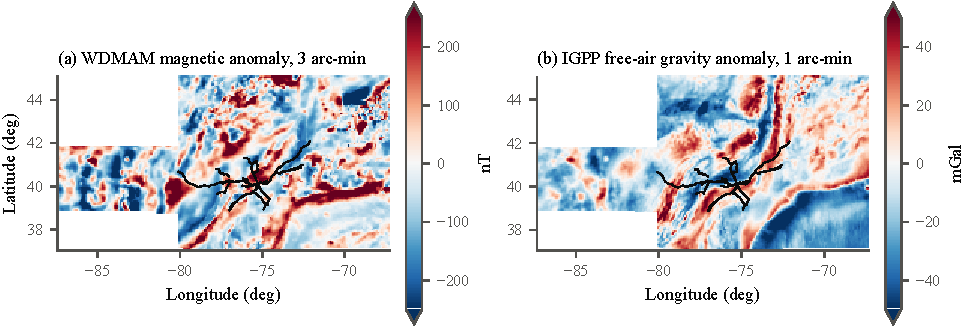
\includegraphics[width=\textwidth]{fig_maps}
  \caption{The Anomaly Maps and the 27 MEMS-Nav Tracks. Each panel is the union of the map tiles cropped around the individual drives.}
  \label{fig:maps}
\end{figure}

\subsection{Measurement Models}

The smartphone records a three-axis gravity vector and a three-axis magnetic field, and only their norms enter the anomaly. Two properties of these vectors matter below. The gravity vector \(\mathbf{g}_\text{obs}\) is not a raw accelerometer measurement but the operating system's fused estimate of gravity, intended to exclude the vehicle's kinematic acceleration. The magnetic vector \(\mathbf{B}_\text{obs}\) is the operating system's calibrated field, from which a hard-iron offset estimated by the phone has already been removed. The gravity anomaly, in mGal, is
\begin{equation}
  z_g = 10^{5}\left[\lVert\mathbf{g}_\text{obs}\rVert - \gamma(L, h) + E\right], \qquad
  E = 2\omega_{ie} v_E \cos L + \frac{v_N^2}{R_N + h} + \frac{v_E^2}{R_E + h},
  \label{eqn:gravity-anomaly-obs}
\end{equation}
where \(\gamma\) is Somigliana normal gravity at the observation height, \(E\) is the E\"{o}tv\"{o}s correction, the vertical component of the Coriolis and transport-rate accelerations of a platform moving over the rotating Earth \citep{groves_ch5}, and \(R_N\) and \(R_E\) are the meridian and transverse radii of curvature. A moving gravimeter reads less than local gravity by \(E\), so the correction is added. Because \(h\) is ellipsoidal height, \(z_g\) is strictly a gravity disturbance, which differs from the map's free-air anomaly by a near-constant offset that the bias state absorbs. The magnetic anomaly, in nT, is
\begin{equation}
  z_m = \lVert\mathbf{B}_\text{obs}\rVert - F_\text{WMM}(L, \lambda, h, t),
  \label{eqn:magnetic-anomaly-obs}
\end{equation}
where \(F_\text{WMM}\) is the total intensity of the World Magnetic Model at the epoch of the recording, WMM2020 before 2025 and WMM2025 thereafter \citep{wmm2020, wmm}. Both anomalies are formed at the filter's own estimate of position and velocity, and both are predicted as the map value at the estimated position plus a bias state,
\begin{equation}
  \hat{z} = \mathcal{M}(L, \lambda) + b,
  \label{eqn:anomaly-prediction}
\end{equation}
where \(\mathcal{M}\) is the bilinear interpolation of the map. In the Kalman filters \(b\) follows a random walk; in the RBPF it is the sum \(V_k + c_k\) of \Cref{eqn:rbpf-partition}. Anomaly updates are applied once per second, without an innovation gate, as a single two-dimensional update with diagonal \(\mathbf{R}\) when both channels are enabled.

\paragraph{EKF.} Because \(\hat{z}\) depends on position only, the measurement Jacobian is non-zero only in the latitude and longitude columns and the bias column. The two map derivatives are central finite differences of the bilinear interpolant with a step of \(10^{-6}\)~deg, converted from degrees to the radians the state holds. This Jacobian omits the dependence of the observation itself on the state, through the reference fields and the motion correction. Along these drives the WMM intensity changes by about 5~nT/km, normal gravity by about 0.8~mGal/km northward, the E\"{o}tv\"{o}s term by about 11~mGal per m/s of east velocity, and normal gravity by 0.31~mGal per meter of height. The effective Jacobian is the derivative of the prediction minus the observation, so for the magnetic channel the map and WMM gradients can reinforce or cancel, and the sign of the effect of this omission on navigation error is not known without a complete-model comparison, which is left to future work.

\paragraph{UKF.} The UKF passes its sigma points through \Cref{eqn:anomaly-prediction}, so the map nonlinearity enters through the spread of the sigma points rather than through a local gradient.

\paragraph{RBPF.} The observation is formed once at the ensemble mean, as the Kalman filters form it, and the residual of particle \(i\) is
\begin{equation}
  r^i = z - \left[\mathcal{M}(\bar{L} + \delta L^i,\,\bar{\lambda} + \delta\lambda^i) + \bar{V} + \bar{c} + V^i + c^i\right],
  \label{eqn:rbpf-map-residual}
\end{equation}
where barred quantities are the nominal. The map is evaluated at each particle's own horizontal position, which is where the particle filter could, in principle, represent a multimodal likelihood that a Gaussian filter cannot. A particle that leaves the map tile receives zero weight. The dependence of the gravity observation on velocity through the E\"{o}tv\"{o}s term is not modeled in \(\mathbf{C}\).

\subsection{Error Models}
\label{sec:error-models}

\paragraph{Smartphone observations.} The error model of each smartphone observation is measured from the data. For each drive, \Cref{eqn:gravity-anomaly-obs} or \Cref{eqn:magnetic-anomaly-obs} is formed along the recorded GNSS track and differenced against the map at the same positions. The pooled median residual seeds the bias state, the median of the within-drive robust standard deviations sets \(\sqrt{R}\), and the spread of the per-drive medians sets the bias prior, which the bias random walk rebuilds over one hour. The signal-to-noise ratio of drive \(j\) is
\begin{equation}
  \mathrm{SNR}_j = \frac{\sigma_{\mathcal{M},j}}{1.4826\,\mathrm{MAD}(\mathbf{r}_j)},
  \label{eqn:snr}
\end{equation}
where \(\sigma_{\mathcal{M},j}\) is the standard deviation of the map along the drive, \(\mathbf{r}_j\) the residuals, and MAD the median absolute deviation. Because the spread is taken about the drive's own median, a bias that is constant over the drive does not lower the SNR; it is left to the bias state. An SNR below one means that the residual scatter exceeds the variation of the map along the track, so that a single measurement cannot distinguish one position on the track from another. Calibrating \(\mathbf{R}\) against the GNSS track is a best case for the filter; it cannot make an observation more informative than it is.

\begin{table}[htb]
  \caption{Anomaly Error Models. Smartphone values are measured from the residuals against the maps; dedicated-sensor values are taken from the datasheet models of \Cref{tab:sensors}. Signal \(\sigma\) is the median over drives of \(\sigma_{\mathcal{M},j}\); SNR is the median over drives of \Cref{eqn:snr}, with the best drive in parentheses.}
  \label{tab:error-model}
  \centering
  \small
  \begin{tabular}{llrrrrl}
\toprule
Sensor & Field & Bias seed & \(\sqrt{R}\) & Prior \(\sigma\) & Signal \(\sigma\) & SNR \\
\midrule
Smartphone & Gravity (mGal) & 841.7 & 131.1 & 252.8 & 14.3 & 0.13 (0.38) \\
Smartphone & Magnetic (nT) & 23{,}342.7 & 7{,}537.3 & 45{,}902.2 & 73.3 & 0.01 (0.04) \\
\midrule
ADXL355 & Gravity (mGal) & 0.0 & 54.8 & 8{,}826.0 & 14.3 & 0.26 (0.48) \\
RM3100 & Magnetic (nT) & 0.0 & 3.9 & 17.1 & 73.3 & 18.4 (56.7) \\
\bottomrule
\end{tabular}

\end{table}

\paragraph{Dedicated sensors.}
\label{sec:dedicated-sensors}
To separate the observation from the estimator and the IMU, a second set of inputs replaces only the norms of the recorded gravity and magnetic vectors with simulated readings of two commercially available low-cost sensors (\Cref{tab:sensors}). For every record the synthetic reading is the reference field at the recorded GNSS position and velocity, plus the map at that position, plus a sensor error; it is constructed by inverting \Cref{eqn:gravity-anomaly-obs,eqn:magnetic-anomaly-obs}, so that a filter at the recorded GNSS state recovers exactly the map value plus the sensor error. Vector directions are kept, so the heading observation, the IMU data, the barometer, the degraded GNSS stream, the filter configurations, and the random seed are unchanged. The magnetometer is a PNI RM3100 magneto-inductive sensor \citep{rm3100}, whose noise averaged to the 10~Hz record rate is 3.9~nT, consistent with the 4.7~nT at 10~Hz measured by \citet{regoli2018investigation}. The gravimeter is an Analog Devices ADXL355 MEMS accelerometer read as a scalar gravimeter \citep{adxl355}, whose noise density of 25~\(\mu\)g/\(\sqrt{\text{Hz}}\) gives 55~mGal per record. Each sensor also draws a turn-on bias per drive, a Gauss--Markov bias instability, and a residual temperature term; the temperature terms assume 90\% compensation and a cabin temperature varying by 1~\(^\circ\)C, and are the only parameters not taken from a datasheet or a published characterization. Gravity readings are withheld wherever the bracketing GNSS fixes are more than 2~s apart, since the velocity needed to invert the E\"{o}tv\"{o}s term cannot be interpolated across a longer gap. The filters use the datasheet error model directly: a zero bias seed, \(\sqrt{R}\) equal to the per-record white noise, and a bias prior and random walk matched to the turn-on, instability, and temperature terms. In the RBPF the bias splits into a variation of 11.4~mGal with an 826-s correlation time and 1.71~nT with 3{,}597~s, and a constant that takes the remainder of the prior.

Installation is deliberately ideal: the vehicle's magnetic field is absent, its kinematic vertical acceleration is removed exactly, and the maps are exact. The dedicated-sensor arm is therefore a sensor-limited best case rather than a prediction of a fielded system, and any benefit it shows is an upper bound on what the same sensor would provide in a vehicle.

\begin{table}[htb]
  \caption{Error Models of the Simulated Dedicated Sensors, per 10~Hz Record. Gauss--Markov terms are given as a standard deviation and a correlation time.}
  \label{tab:sensors}
  \centering
  \small
  \begin{tabular}{lll}
    \toprule
    Error term & ADXL355 gravimeter & RM3100 magnetometer \\
    \midrule
    Unit price & \$77 & \$25 \\
    White noise & 54.8~mGal & 3.92~nT \\
    Turn-on bias & 8{,}826~mGal (9~mg) & 17.0~nT \\
    Bias instability & 5.6~mGal, 300~s & 1.7~nT, 3{,}600~s \\
    Temperature & 10.0~mGal, 1{,}800~s & 0.05~nT, 1{,}800~s \\
    \bottomrule
  \end{tabular}
\end{table}

\Cref{fig:residuals} compares the residual spread of both sets of observations with the variation of the map along the tracks. The smartphone's noise exceeds the map signal by an order of magnitude for gravity and by two orders of magnitude for the magnetic field, and no drive reaches an SNR of one in either channel (\Cref{tab:error-model}). The simulated RM3100 reaches an SNR above one on 24 of 27 drives. The simulated ADXL355 doubles the smartphone's gravity SNR but, at 0.26, still falls well short of one. Before any filter is run, the error models therefore predict no benefit from the smartphone observations or the ADXL355, and some benefit from the RM3100.

\begin{figure}[htb]
  \centering
  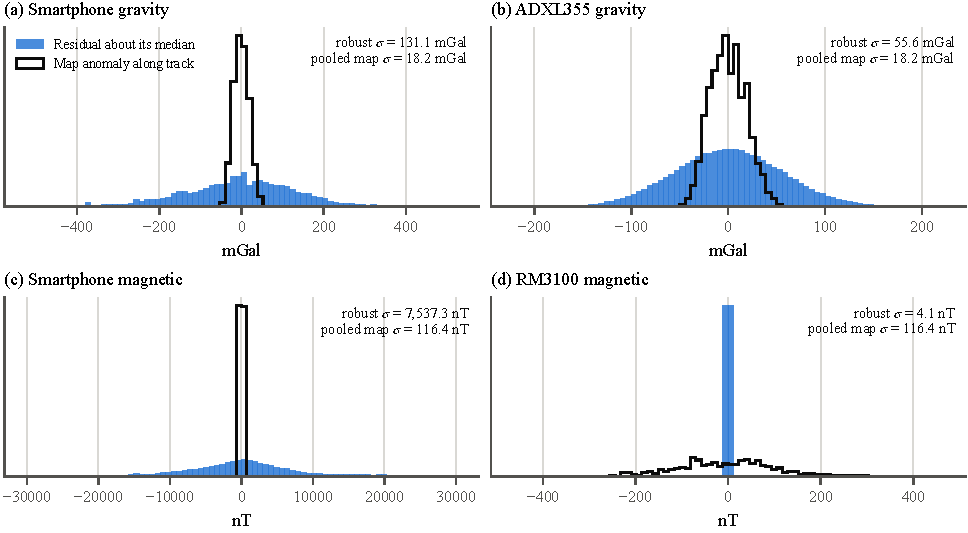
\includegraphics[width=\textwidth]{fig_residuals}
  \caption{Residuals of the Anomaly Observations Against the Maps. Each drive's residuals are taken about their own median; the outline is the map anomaly along the same tracks, each drive's mean removed. The robust \(\sigma\) is the pooled \(1.4826\,\mathrm{MAD}\) of the residuals; the pooled map \(\sigma\) is larger than the per-drive median signal \(\sigma\) of \Cref{tab:error-model} because it mixes drives.}
  \label{fig:residuals}
\end{figure}

\section{Data and Experimental Design}
\label{sec:experiment}

\subsection{The MEMS-Nav Drives}

The data are the MEMS-Nav recordings \citep{mems-nav-dataset}, made with the Sensor Logger application on seven models of Android and iOS smartphone mounted in passenger cars, mostly on highways in the Mid-Atlantic and northeastern United States between August 2023 and November 2025 (\Cref{fig:maps}). Each recording contains three-axis specific force, angular rate, and magnetic field, the operating system's gravity vector and attitude, barometric pressure and relative altitude, and GNSS position, velocity, and reported accuracies. The 29 raw recordings are resampled to a 10~Hz record rate, which gives 10~Hz inertial propagation; GNSS remains at the roughly 1~Hz rate at which it was logged, and its columns are left empty between fixes rather than interpolated. Recordings are split wherever the IMU stream has a gap longer than 5~s, and segments shorter than 300~s are discarded, which yields the 27 drives of \Cref{tab:dataset}.

\begin{table}[htb]
  \caption{The 27 MEMS-Nav Drives}
  \label{tab:dataset}
  \centering
  \small
  \begin{tabular}{lrr}
\toprule
 & Distance & Duration \\
\midrule
Trajectories & 27 &  \\
Total & 4{,}338~km & 55.3~h \\
Median & 141.8~km & 1.74~h \\
Mean & 160.7~km & 2.05~h \\
Range & 1.1--497.2~km & 0.11--4.95~h \\
\bottomrule
\end{tabular}

\end{table}

No independent reference trajectory exists for these drives, so every error in this paper is the horizontal great-circle distance between the filter's estimate and the recorded GNSS fix, evaluated at the records that carry one, and summarized per drive as a root-mean-square error (RMSE). The recorded GNSS is itself in error by a few meters, which limits the precision with which small differences can be resolved but applies equally to every configuration. One drive, 2025-06-14 21:17:02, is of poor quality: it has 197 GNSS fixes over less than ten minutes, with a median reported horizontal accuracy of 12.2~m and nine fixes reporting an accuracy of 999~m or more. It is retained, and it is the worst drive for every filter.

\subsection{Experimental Design}

Each of the 27 drives was processed by each of the three filters in five configurations: full GNSS, degraded GNSS, and degraded GNSS with gravity, magnetic, or combined anomaly aiding. The aided configurations were run twice, once with the smartphone's own observations and once with the simulated dedicated sensors, giving \(27 \times 3 \times (2 + 2 \times 3) = 648\) runs. Within a pair, the aided and unaided runs share the filter, its initialization and process noise, the barometric and heading updates, the degraded GNSS stream, and the random seed, and differ only in the map-bias states and the anomaly updates.

Because the degraded-GNSS error varies by almost an order of magnitude across drives (\Cref{fig:baselines}), each aided run is scored by the ratio of its horizontal RMSE to that of the same filter's unaided run on the same drive; a ratio below one is an improvement. The ratios of a configuration are summarized by their median with a 95\% percentile bootstrap interval (10{,}000 resamples) \citep{efron1993bootstrap}, by the number of drives improved and worsened, and by a two-sided Wilcoxon signed-rank test on the paired differences \citep{wilcoxon1945individual}. A drive enters a comparison only if both of its runs completed. A run is stopped if the filter's speed exceeds 5{,}000~m/s; this health limit is deliberately loose so that MEMS-grade runs can drift to completion, which also makes completion weak evidence that a run stayed healthy.

The smartphone and dedicated-sensor inputs differ only in the norms of the gravity and magnetic vectors, so their unaided runs should coincide. They do for the UKF, whose degraded-GNSS RMSE changes by more than 1\% on \numsensukfcount{} of \numsensukfn{} drives, but not for the other two filters: the magnetic vector feeds the heading observation, and the last-bit difference introduced by rescaling it changes the EKF's RMSE by more than 1\% on \numsensekfcount{} of \numsensekfn{} drives (by up to \numsensekfmaxm~m) and the RBPF's on \numsensrbpfcount{} of the \numsensrbpfn{} drives common to both sets, with a median change of \numsensrbpfmedianpct\%. Each set of aided runs is therefore compared with its own unaided runs. The sensitivity of the RBPF to this perturbation is itself a result (\Cref{sec:results-rbpf}).

The dedicated-sensor and unaided runs read the configuration files as committed at \texttt{2a40f1e} of \texttt{strapdown-rs}, with seed 42; the revision of the binary that executed them was not recorded. The configurations of the smartphone-sensor runs were not archived; their filter settings are believed to match, but this has not been verified. The analysis scripts that produce every table, figure, and quoted statistic from the run outputs are available as described at the end of the paper.

\section{Results}
\label{sec:results}

\newcommand{\phonegravcorr}{-0.055}
\newcommand{\phonegravcorrn}{27}
\newcommand{\phonegravpinned}{85}
\newcommand{\phonegravslope}{-0.02}
\newcommand{\phonemagamplitude}{14.7}
\newcommand{\phonemagmapsd}{72}
\newcommand{\phonemagn}{25}
\newcommand{\phonemagrsq}{52}
\newcommand{\phonemagspread}{8.3}


\subsection{Unaided Baselines}
\label{sec:results-baselines}

\Cref{tab:baselines} and \Cref{fig:baselines} give the horizontal RMSE of each unaided filter with full and degraded GNSS. With full GNSS the three filters track the recorded solution closely, with medians of \numekffullmedian~m for the EKF, \numukffullmedian~m for the UKF, and \numrbpffullmedian~m for the RBPF, consistent with loosely coupled integration of consumer-grade sensors. The poor-quality 2025-06-14 drive is the worst for all three. The RBPF also diverges on one drive, 2023-08-04, that both Kalman filters hold to about 4~m.

With one fix per minute, the medians rise to \numekfdegradedmedian~m for the EKF and \numukfdegradedmedian~m for the UKF, a factor of about a hundred, and no drive falls below 280~m. The two Kalman filters agree to within 5\% on most drives, and where they differ the UKF is usually the better. This two-order-of-magnitude gap between degraded and full GNSS is what anomaly aiding is asked to close. The RBPF does not maintain a solution under this schedule: its horizontal RMSE exceeds 10~km on 24 of the 25 drives that ran to completion, with a median of \numrbpfdegradedmedian, and two drives were stopped by the 5{,}000~m/s health limit. \Cref{sec:results-rbpf} examines this failure.

\begin{table}[htb]
  \caption{Horizontal RMSE of the Unaided Filters Across Drives. \(n\) is the number of drives that ran to completion.}
  \label{tab:baselines}
  \centering
  \small
  \begin{tabular}{llrrrrr}
\toprule
Filter & GNSS & \(n\) & Median (m) & Mean (m) & Max (m) & Vert.\ median (m) \\
\midrule
EKF & Full & 27 & 4.1 & 24.0 & 539.2 & 1.6 \\
 & Degraded & 27 & 440.4 & 601.7 & 2{,}436.1 & 23.4 \\
\midrule
UKF & Full & 27 & 4.0 & 24.0 & 542.8 & 1.6 \\
 & Degraded & 27 & 430.4 & 577.1 & 3{,}115.4 & 24.0 \\
\midrule
RBPF & Full & 27 & 1.9 & 181.7 & 3{,}628.5 & 1.6 \\
 & Degraded & 25 & 664.6~km & 900.4~km & 2{,}706.6~km & 409.5 \\
\bottomrule
\end{tabular}

\end{table}

\begin{figure}[htb]
  \centering
  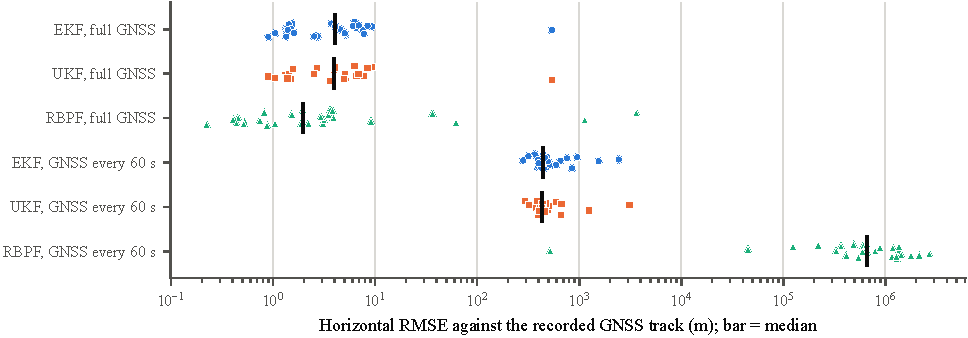
\includegraphics[width=\textwidth]{fig_baselines}
  \caption{Horizontal RMSE of Each Unaided Filter on Each Drive, with Full GNSS and with One Fix per Minute. Bars mark the medians; the horizontal axis is logarithmic.}
  \label{fig:baselines}
\end{figure}

\subsection{Aiding with the Smartphone's Own Observations}
\label{sec:results-phone}

\Cref{tab:aiding} summarizes the paired comparisons for the two Kalman filters, and \Cref{fig:ratios} shows the per-drive ratios. With the smartphone's observations, neither filter changes measurably under any aiding channel. The median ratio lies between 1.000 and 1.001 in all six configurations, no 95\% interval admits a change larger than 0.3\%, and no comparison is significant (\(p \geq 0.13\)). The largest median per-drive change is an increase of half a meter on a degraded error of several hundred meters. The individual ratios that depart visibly from one in \Cref{fig:ratios}(a) belong to the EKF on a few drives whose degraded-GNSS solution is sensitive to small perturbations of any kind (\Cref{sec:experiment}); they fall on both sides of one. \Cref{fig:example}(a) shows a representative drive, on which the aided and unaided EKF errors are indistinguishable at the scale of the dedicated-sensor result.

This is the outcome the error models predict. With a measurement noise one to two orders of magnitude larger than the map signal, the Kalman gain of the anomaly update is close to zero, and both filters correctly assign the observation almost no weight.

\begin{table}[htb]
  \caption{Effect of Anomaly Aiding on the Kalman Filters Under Degraded GNSS. Ratio is the median over 27 drives of the aided to unaided horizontal RMSE of the same filter, with its 95\% bootstrap interval; B/W counts drives improved and worsened; \(p\) is from a two-sided Wilcoxon signed-rank test. Ratios below one are improvements.}
  \label{tab:aiding}
  \centering
  \small
  \setlength{\tabcolsep}{4pt}
  \begin{tabular}{llccc@{\hspace{1.2em}}ccc}
\toprule
 & & \multicolumn{3}{c}{Smartphone observations} & \multicolumn{3}{c}{Dedicated sensors} \\
\cmidrule(lr){3-5}\cmidrule(lr){6-8}
Filter & Aiding & Ratio [95\% CI] & B/W & \(p\) & Ratio [95\% CI] & B/W & \(p\) \\
\midrule
EKF & Gravity & 1.001 [1.000, 1.002] & 7/20 & 0.18 & 1.005 [1.001, 1.013] & 8/19 & 0.17 \\
 & Magnetic & 1.000 [1.000, 1.000] & 12/15 & 0.93 & 0.891 [0.866, 0.907] & 25/2 & \(<10^{-3}\) \\
 & Combined & 1.001 [1.000, 1.002] & 8/19 & 0.46 & 0.890 [0.880, 0.913] & 24/3 & \(<10^{-3}\) \\
\midrule
UKF & Gravity & 1.001 [1.000, 1.003] & 9/18 & 0.13 & 1.011 [1.000, 1.013] & 8/19 & 0.049 \\
 & Magnetic & 1.000 [1.000, 1.000] & 13/14 & 0.86 & 0.901 [0.884, 0.905] & 26/1 & \(<10^{-3}\) \\
 & Combined & 1.001 [1.000, 1.002] & 8/19 & 0.14 & 0.899 [0.883, 0.929] & 26/1 & \(<10^{-3}\) \\
\bottomrule
\end{tabular}

\end{table}

\begin{figure}[htb]
  \centering
  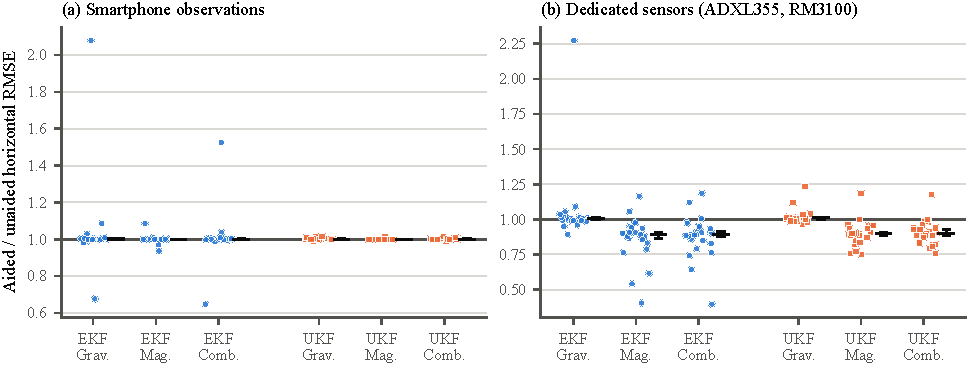
\includegraphics[width=\textwidth]{fig_ratios}
  \caption{Per-Drive Ratio of Aided to Unaided Horizontal RMSE for the Kalman Filters. Points are drives; the black marks are the median and its 95\% bootstrap interval. The vertical scales of the two panels differ.}
  \label{fig:ratios}
\end{figure}

\subsection{Why the Smartphone Observations Carry No Map Information}
\label{sec:results-cause}

The null result is explained by how the smartphone forms its readings, without reference to any filter (\Cref{fig:phone-sensors}).

\paragraph{Gravity.} The recorded vector is the operating system's fused estimate of gravity, and its norm is pinned to a device constant: on the median drive, \phonegravpinned\% of records lie within 1~mGal of the drive's maximum, which is 9.81000~m/s\(^2\) on the Google Pixel devices and the standard gravity of 9.80665~m/s\(^2\) on most others. The excursions below that ceiling follow the vehicle's dynamics rather than the map. Averaged over 60-s blocks, the norm correlates with the map at a median of \(r = \phonegravcorr\) with a regression slope of \(\phonegravslope\), where a gravimeter would give a slope of one. Because the norm is effectively constant, the anomaly of \Cref{eqn:gravity-anomaly-obs} reduces to a function of the filter's own latitude, height, and velocity, through normal gravity and the E\"{o}tv\"{o}s term: it is a biased velocity pseudo-measurement rather than a map observation. The raw accelerometer offers no alternative. Projected onto the vertical, corrected for normal gravity, the E\"{o}tv\"{o}s term, and barometrically derived vertical acceleration, and averaged over 120 to 600~s, its residual remains 50 to 90 times the map signal \citep{brodovsky2026dissertation}.

\paragraph{Magnetic field.} The magnetometer is dominated by the vehicle. A smartphone fixed in a car yaws only with the car, so a field fixed to the vehicle adds a heading-dependent term to the measured intensity that a scalar bias state cannot follow. Fitting the intensity anomaly of \Cref{eqn:magnetic-anomaly-obs} to the vehicle's course over ground explains a median \phonemagrsq\% of its variance, with a heading-dependent amplitude of \phonemagamplitude~\(\mu\)T. The intensity varies along a drive with a median standard deviation of \phonemagspread~\(\mu\)T, against \phonemagmapsd~nT for the map along the same track. This is despite the operating system's own calibration, which removes a hard-iron offset of 67 to 325~\(\mu\)T per recording \citep{brodovsky2026dissertation}.

\begin{figure}[htb]
  \centering
  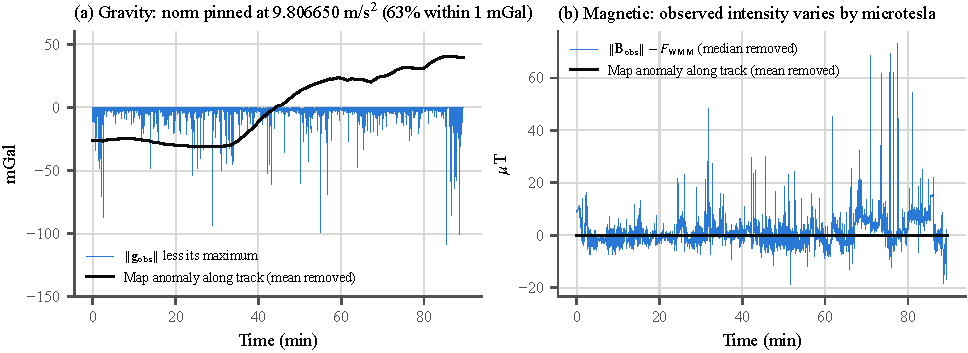
\includegraphics[width=\textwidth]{fig_phone_sensors}
  \caption{The Smartphone's Gravity and Magnetic Observations on Drive 2025-03-01 16:46:39, Against the Map Along the Same Track. (a) The norm of the reported gravity vector, in mGal below its maximum; (b) the magnetic intensity anomaly, in \(\mu\)T. Both maps are drawn with their mean removed and on the same scale as the observation.}
  \label{fig:phone-sensors}
\end{figure}

The consequence for navigation is captured by a localization bound: the measurement noise divided by the median gradient of the map along the track, which is the position uncertainty that a single update can resolve. \Cref{fig:bound} gives this bound for each observation. For the smartphone it is about 90~km for gravity and 1{,}200~km for the magnetic field, two to three orders of magnitude larger than the 0.44~km median error of the degraded solution. An observation that resolves position far less precisely than the solution already holds cannot improve it.

\begin{figure}[htb]
  \centering
  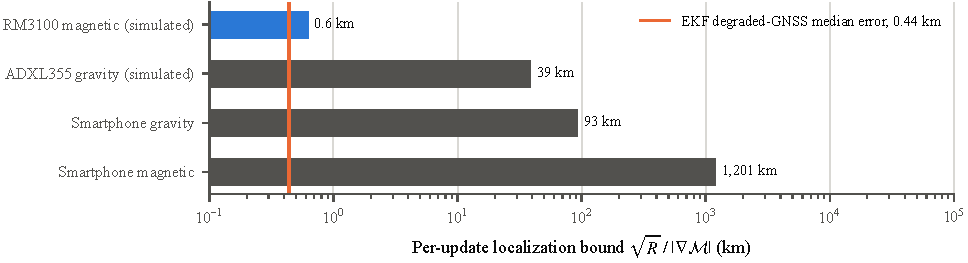
\includegraphics[width=\textwidth]{fig_bound}
  \caption{Per-Update Localization Bound of Each Observation: Measurement Noise \(\sqrt{R}\) Divided by the Median Map Gradient Along the 27 Tracks (1.41~mGal/km, 6.28~nT/km). The vertical line is the median horizontal RMSE of the unaided EKF under degraded GNSS.}
  \label{fig:bound}
\end{figure}

\subsection{Aiding with Dedicated Sensors}
\label{sec:results-dedicated}

The right half of \Cref{tab:aiding} and \Cref{fig:ratios}(b) give the same comparisons with the simulated dedicated sensors, with the IMU, the degraded GNSS, the filters, and the seed unchanged. With the RM3100 magnetometer, magnetic aiding improves the EKF on \numdedicatedekfmagbetter{} of 27 drives and the UKF on \numdedicatedukfmagbetter{}, with median ratios of \numdedicatedekfmagratio{} and \numdedicatedukfmagratio{} (\(p < 10^{-3}\) for both) and median reductions of \numdedicatedekfmagdmed~m and \numdedicatedukfmagdmed~m. Because the full-GNSS error is only a few meters, a ratio of 0.89 closes about a tenth of the gap between degraded and full-GNSS performance. \Cref{fig:example}(b) shows the drive whose EKF ratio lies at the median of the dataset: the aided error is lower for most of the drive, with short intervals in which it is higher, and the RMSE falls by 52~m. Gravity aiding with the ADXL355 does not help either filter; the EKF ratio is \numdedicatedekfgravratio{} and the UKF ratio \numdedicatedukfgravratio{}, both worse on 19 of 27 drives, and only the UKF result reaches marginal significance (\(p = \numdedicatedukfgravp\)). Combined aiding performs as magnetic aiding alone, because both filters assign the uninformative gravity channel almost no weight.

\begin{figure}[htb]
  \centering
  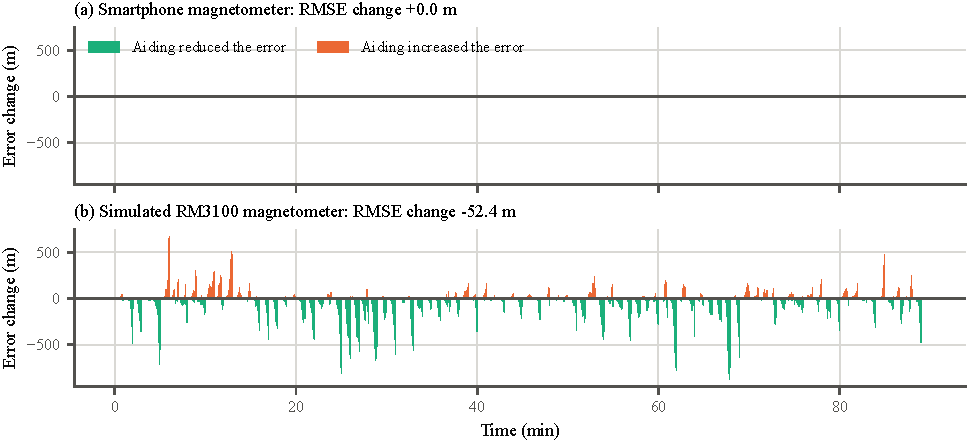
\includegraphics[width=\textwidth]{fig_example}
  \caption{Aided Minus Unaided Horizontal Error of the EKF on Drive 2025-03-01 16:46:39, with Magnetic Aiding from (a) the Smartphone Magnetometer and (b) the Simulated RM3100. Both panels share one vertical scale. Green intervals are those in which aiding reduced the error.}
  \label{fig:example}
\end{figure}

The same filters, inertial data, and GNSS stream that were unaffected by the smartphone observations therefore benefit consistently once the magnetic observation carries map information. Because the IMU was held fixed, this places the cause of the smartphone result in the observations rather than in the consumer-grade inertial sensor or the estimators. The size of the gain agrees with the localization bound of \Cref{fig:bound}: the RM3100's bound of about 0.6~km is comparable to the 0.44~km degraded error, so each update constrains position only to about the accuracy the INS already holds, which predicts a consistent but modest improvement. The ADXL355's bound of about 40~km predicts none.

\subsection{The Particle Filter Under Degraded GNSS}
\label{sec:results-rbpf}

The RBPF loses track under the 60-s GNSS schedule with or without aiding, so the effect of aiding on it cannot be assessed. \Cref{tab:rbpf} lists its paired results for completeness; the aided and unaided errors are both hundreds of kilometers, set by the divergence rather than by the anomaly measurement, and the ratios are not interpretable. \Cref{fig:rbpf} shows the failure on the example drive. Within the first minutes the RBPF's error leaves the range of the Kalman filters' and never returns, while its reported horizontal standard deviation stays at tens to hundreds of meters, the same order as the EKF's actual error. Across the drives, the error first exceeds 10~km after a median of 6~minutes, and over the second half of each drive the reported standard deviation has a median of 74~m against a median error of 880~km. The filter is not merely inaccurate but confidently wrong by four orders of magnitude.

\begin{table}[htb]
  \caption{Paired Results of the RBPF Under Degraded GNSS, Reported for Completeness. Both aided and unaided runs have diverged, so the comparison does not measure the anomaly measurement. \(n\) counts drives on which both runs completed.}
  \label{tab:rbpf}
  \centering
  \small
  \begin{tabular}{llrrcc}
\toprule
Observations & Aiding & \(n\) & Unaided median & Aided median & B/W \\
\midrule
Smartphone & Gravity & 25 & 801.7~km & 750.2~km & 14/11 \\
 & Magnetic & 26 & 817.9~km & 686.8~km & 12/14 \\
 & Combined & 25 & 801.7~km & 794.4~km & 13/12 \\
\midrule
Dedicated & Gravity & 25 & 664.7~km & 844.7~km & 11/14 \\
 & Magnetic & 25 & 664.7~km & 730.8~km & 10/15 \\
 & Combined & 25 & 664.7~km & 749.0~km & 18/7 \\
\bottomrule
\end{tabular}

\end{table}

\begin{figure}[htb]
  \centering
  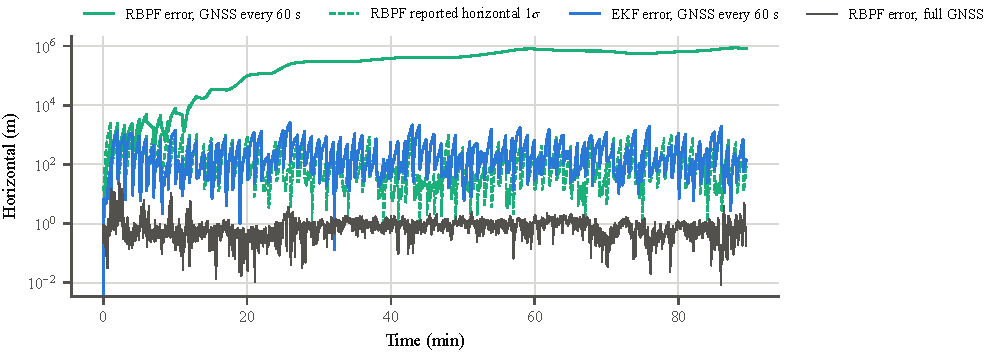
\includegraphics[width=\textwidth]{fig_rbpf}
  \caption{Horizontal Error and Reported Uncertainty of the Unaided RBPF on Drive 2025-03-01 16:46:39 with One GNSS Fix per Minute, Against the Unaided EKF on the Same Stream and the RBPF with Full GNSS. The vertical axis is logarithmic.}
  \label{fig:rbpf}
\end{figure}

That signature is particle deprivation. Horizontal position lives only in the particles, so a GNSS fix can correct it only by reweighting and resampling among them. Once the drift between fixes carries the true error outside the cloud, which is tens of meters wide, each fix can move the estimate by at most about one cloud width, and the filter never re-acquires. With a fix every second the drift never leaves the cloud, which is why the same filter has the lowest median error of the three with full GNSS. Why the cloud drifts out in the first place is not established. The RBPF, like the filter of \citet{canciani2017airborne}, estimates no IMU biases, so its nominal drifts between fixes on errors that the Kalman filters estimate and remove; but adding bias states also diverged, so their absence is not a demonstrated cause. A second candidate is the transfer of velocity uncertainty from the shared covariance into the particle spread described in \Cref{sec:rbpf}, which resampling then discards, and which over 60-s epochs may recur at every fix.

The RBPF is also far less repeatable than the Kalman filters. The last-bit change in the heading input that distinguishes the two sets of unaided runs (\Cref{sec:experiment}) changes the RBPF's degraded-GNSS RMSE by more than 1\% on 22 of 25 drives, with a median change of 20\%, against one drive for the EKF and none for the UKF.

\section{Discussion}
\label{sec:discussion}

\subsection{What Decides Whether Anomaly Aiding Helps}

Across four observations, two estimators, and one consumer-grade IMU, the outcome is ordered by a single quantity: the quality of the anomaly measurement relative to the map signal. The two smartphone observations and the ADXL355, whose single-update scales along the map gradient are \boundscaleadxl{} to \boundscalephonemag~km, provide no benefit; the RM3100, whose scale of about \boundscalermthree~km is comparable to the error of the degraded solution, provides a consistent one. The inertial sensor was held fixed throughout, and the EKF and UKF behave alike, so neither the IMU nor the choice between the two Kalman filters is what limits the smartphone result. A better aiding sensor was sufficient to obtain a benefit; whether a better inertial sensor would add to it was not tested here.

The same heuristic gives an indicative requirement for these roads and maps. For a single update to resolve position along the gradient to the \bounddegradedkm~km of the degraded solution, the measurement noise must be below about \boundreqgrav~mGal for gravity and about \boundreqmag~nT for the magnetic field. Because the heuristic ignores the unobserved contour direction, the bias state, and the accumulation of repeated updates, this is an order-of-magnitude target rather than a threshold. A dedicated low-cost magnetometer approaches the magnetic requirement. No MEMS accelerometer approaches the gravity requirement; land-vehicle strapdown gravimetry has reached the milligal level only with navigation-grade inertial sensors, GNSS velocity, and filtering windows of minutes \citep{yu2015sins}. The map is also part of the heuristic. The WDMAM grid, at 3~arc-minutes and referenced to 5~km altitude, retains little structure at the sub-kilometer scale of the position error, and the free-air grid over land is effectively 9~km. Once the sensor is adequate, map resolution becomes the next limit, and higher-resolution regional surveys would lower it.

When the measurement noise greatly exceeds the map signal, the Kalman gain of the anomaly update falls toward zero and the filter effectively ignores the measurement, which is what both Kalman filters did with every observation except the RM3100. The particle filter has the analogous limit: a likelihood that is exactly independent of the state multiplies every weight by the same constant and leaves the normalized weights, and the systematic resampling of equal weights, unchanged. Its departures from that limit come from elsewhere, namely the finite sample of particles, the roughening jitter added after every resampling, and any mismatch between the modeled and actual measurement errors. The divergence of \Cref{sec:results-rbpf} occurs with and without aiding, so it does not show that weak anomaly updates harm the particle filter.

\subsection{The Particle Filter}

The results do not support the expectation, stated in the authors' conference paper, that a particle filter is the estimator best suited to anomaly aiding. Its theoretical advantage is the ability to represent a multimodal posterior, which arises when the position uncertainty spans several correlation lengths of the map. That is not the regime studied here. With a GNSS fix every minute, the median error of the Kalman-filter solution, about 0.44~km, is far smaller than the effective correlation lengths of the maps, about 9~km for gravity and about 30~km for the magnetic field, so the anomaly likelihood is effectively unimodal over the region of uncertainty. The particle filter's advantage should be sought in long outages, where the position uncertainty grows to the scale of the map features, and with a formulation that survives the degraded-GNSS baseline first. Two structural remedies for the deprivation of \Cref{sec:results-rbpf} are standard: applying GNSS position as a Kalman update of the full error state, which needs no particles because it is linear in position, and proposing particles near each fix, as in sensor resetting or a mixture proposal.

Two properties of the implementation would limit the benefit of aiding even without the divergence. The E\"{o}tv\"{o}s term makes the gravity observation depend on velocity, which the Rao-Blackwellized update does not model, so the likelihood can select particles by velocity rather than by position. And each filter treats successive anomaly errors as independent given the state. For the dedicated sensors this matches how the errors were generated, white noise plus a modeled Gauss--Markov bias over an exact map, so repeated observations of the same map feature do add information. For the smartphone observations it does not: the heading-dependent vehicle field that explains about half of the magnetic intensity variance (\Cref{sec:results-cause}) persists for as long as the heading does, so successive errors are correlated in time and the weights and covariances built on them are optimistic. The spatial correlation of the map alone does not imply correlated measurement errors.

\subsection{Limitations}
\label{sec:limitations}

Several limitations bound these conclusions. The reference for every error is the smartphone's own GNSS track; it limits the precision of small differences, but it applies equally to every configuration in a pair. The dedicated-sensor observations are idealized: the vehicle's magnetic field is absent and the maps are exact, so the magnetic improvement is an upper bound on what the same sensor would provide in a vehicle, where the platform field that dominated the smartphone magnetometer would have to be avoided or compensated. Their errors are a single realization, although each drive draws its own, so each paired test is over 27 independent draws. Anomaly errors are modeled as independent between the once-per-second updates; for the smartphone observations, whose vehicle-field error persists with heading, this is optimistic. The Kalman filters' measurement Jacobian omits the reference-field and motion terms of the observation; the direction of the resulting effect on navigation error is not established, and it is common to every configuration. The magnetometer heading observation shared by every run is itself corrupted by the vehicle's field, with errors far larger than its assumed 0.2~rad. Finally, the experiment covers one degradation scenario; a shorter fix interval would shrink the degraded error and, by the heuristic above, the benefit that any given sensor can provide, whereas a longer outage would enlarge both.

\section{Conclusions}
\label{sec:conclusion}

This paper evaluated gravity and magnetic anomaly aiding of a consumer-grade MEMS INS under degraded GNSS with three estimators on 27 drives, pairing every aided run with the same filter's unaided run on an identical measurement stream. It corrects the authors' earlier conference results, which arose from unit errors in the anomaly observation and from comparisons against differing or diverged baselines.

With corrected observations, the gravity and magnetic readings that a vehicle-mounted smartphone already provides carry no map information and provide no benefit to either Kalman filter. The cause is the readings themselves: the gravity norm is pinned to a device constant and the magnetometer is dominated by the vehicle's field, which gives signal-to-noise ratios of 0.13 and 0.01 against the maps. Replacing only those readings with a simulated \$25 RM3100 magnetometer makes magnetic aiding reduce the median error of both the EKF and the UKF by about 10\%, on 25 and 26 of 27 drives, while a simulated \$77 ADXL355 used as a gravimeter does not help. The size of the magnetic gain is consistent with a single-update heuristic, the sensor noise divided by the map gradient. The deciding variable is the quality of the anomaly measurement relative to the map signal, not the estimator and not the inertial sensor; by the same heuristic, an indicative target on these roads and maps is a noise of about \boundreqgrav~mGal or \boundreqmag~nT.

The Rao-Blackwellized particle filter, which has the lowest median error of the three with full GNSS, loses track with one fix per minute with or without aiding, in a manner consistent with particle deprivation, and its results are far less repeatable than those of the Kalman filters. In the regime studied, where the position uncertainty is much smaller than the correlation lengths of the maps, the Kalman filters are the estimators that worked; whether the particle filter can be made to work under sparse GNSS is open.

Four directions follow. A field trial with a dedicated magnetometer mounted away from, or compensated for, the vehicle's field would test whether the simulated gain survives installation. The Kalman filters' measurement Jacobian should include the reference-field and motion terms, and where the anomaly errors are correlated in time, as the smartphone's vehicle field is, that correlation should be modeled or the update interval lengthened to match it. The particle filter needs a formulation that survives sparse GNSS, by updating position linearly or proposing particles near each fix, before its multimodal advantage can be tested in long outages. And the error-state Kalman filter that \texttt{strapdown-rs} provides as its default estimator should be given an anomaly path and evaluated alongside the filters compared here.


\section*{Data and Software Availability}
The navigation software is \texttt{strapdown-rs} \citep{strapdown-rs}, open source under the MIT license at \url{https://github.com/jbrodovsky/strapdown-rs}; the runs reported here used commit \texttt{827db06}, and the configuration files are under \texttt{conf/} in that repository. The MEMS-Nav recordings are archived at \url{https://doi.org/10.5281/zenodo.17582434} \citep{mems-nav-dataset}. The scripts that compute every table, figure, and quoted statistic in this paper from the run outputs are under \texttt{papers/anom\_combined/scripts/} in the same repository.


\section*{Acknowledgments}
The authors thank the volunteers who recorded drives for the MEMS-Nav dataset.

\section*{Conflict of Interest}
The authors declare no potential conflicts of interest.

\printbibliography[title=References]

\end{document}
